\documentclass{article}
\usepackage{fontspec}

% Used to embed Sage code in latex
%\usepackage{sagetex}


% Math Environment
\usepackage{euler}        % Euler font
\usepackage{amsmath}      % Math macros
\usepackage{amssymb}      % Math symbols
\usepackage{unicode-math} % Unicode support

% Physics Environment
\usepackage{physics}


\usepackage[makeroom]{cancel} % Used to cancel terms in algebraic equations
\usepackage{ulem} % Different underline environments
\usepackage{polynom} %Polynomial long division

% Typesetting Rules
\setlength\parindent{0em}
\setlength\parskip{0.618em}
\usepackage[a4paper,lmargin=1in,rmargin=1in,tmargin=1in,bmargin=1in]{geometry}
\setmainfont[Mapping=tex-text]{Helvetica Neue LT Std 45 Light}

% Common Macros
\newcommand\N{\mathbb{N}}
\newcommand\Z{\mathbb{Z}}
\newcommand\Q{\mathbb{Q}}
\newcommand\R{\mathbb{R}}
\newcommand\C{\mathbb{C}}
\newcommand\A{\mathbb{A}}
\def\res{\mathop{\text{Res}}\limits}

% Color
\usepackage[dvipsnames]{xcolor}
\usepackage{pagecolor}
% \definecolor{DeepMossGreen}{HTML}{394820}
% \pagecolor{DeepMossGreen}
% \color{Goldenrod}

\usepackage{graphicx}

\begin{document}

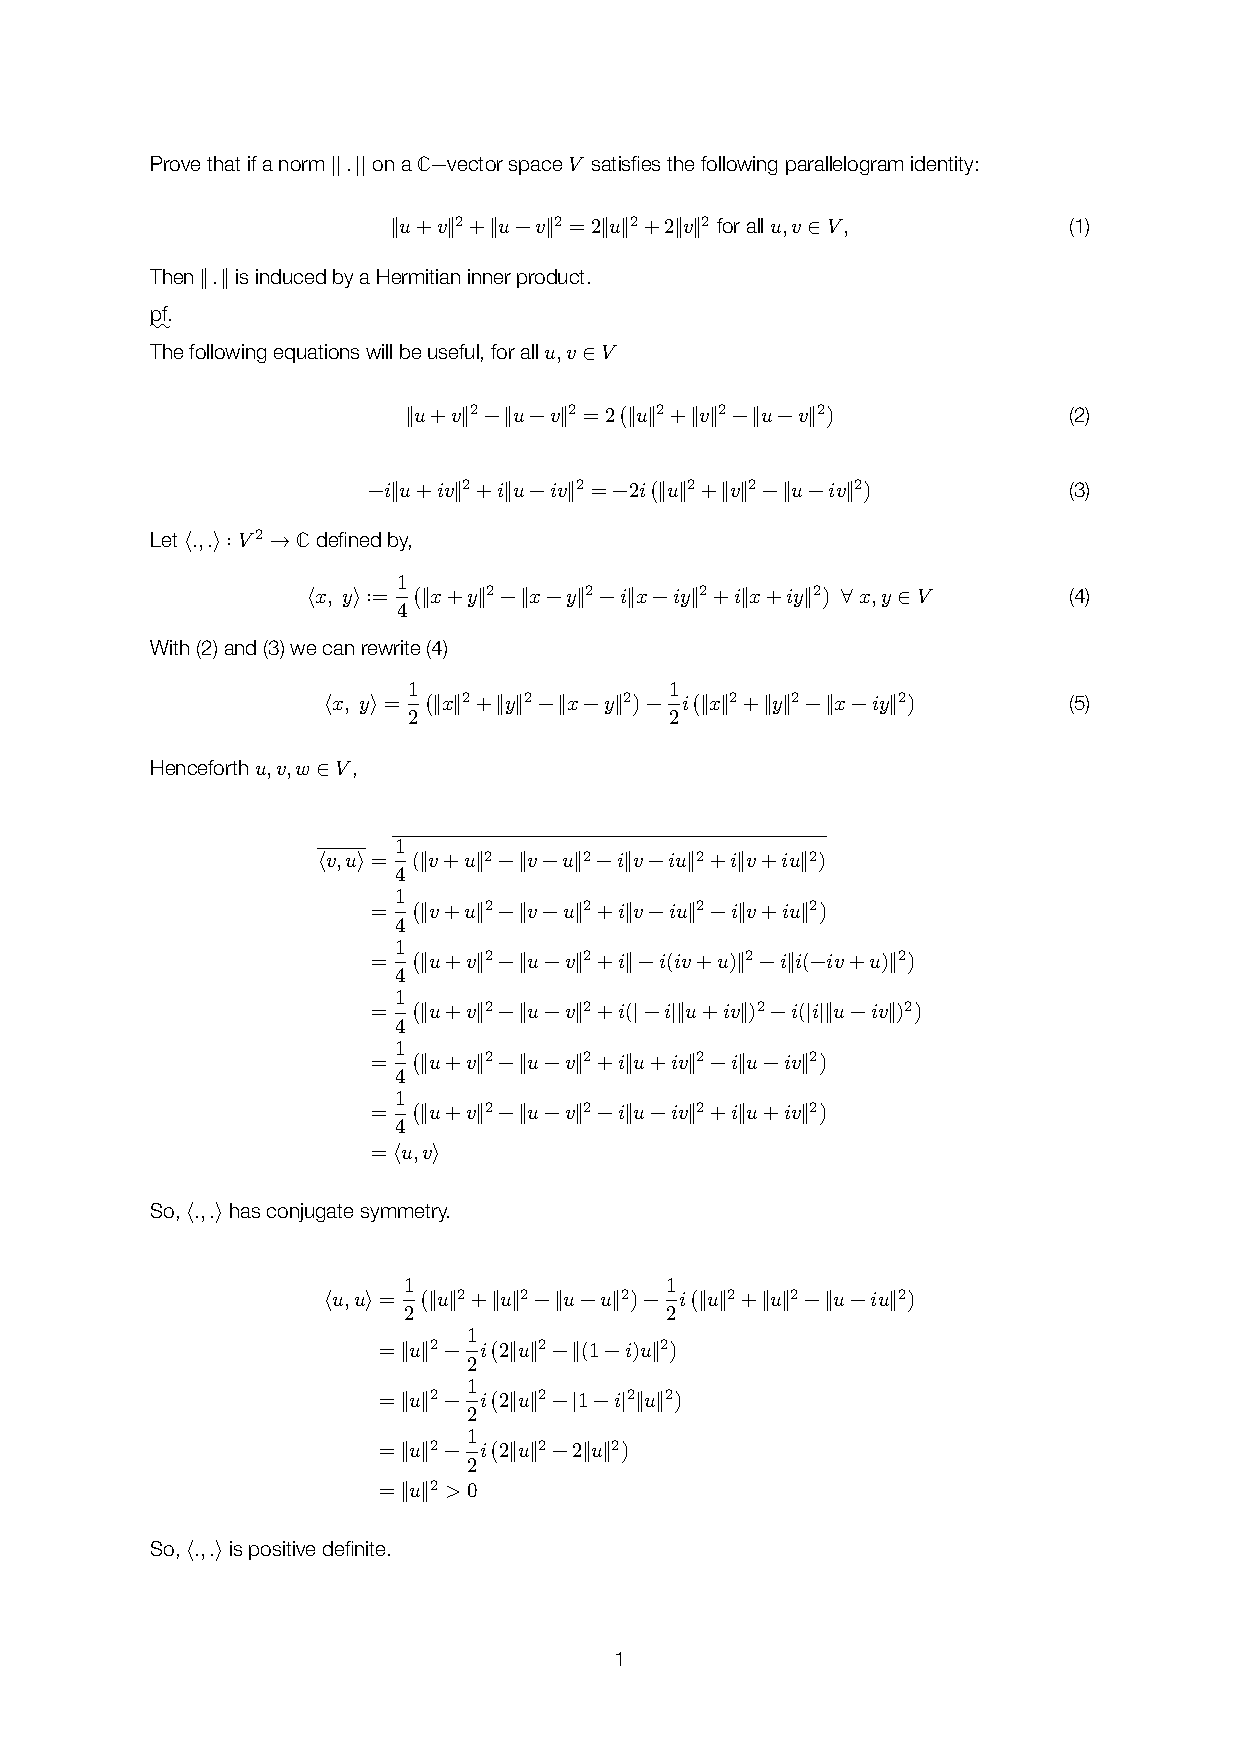
\includegraphics[width=\textwidth]{q1.png}

\uwave{slu.}

Let,$r,\theta \in \R: r>0$, and $ 0<\theta \leq 2\pi$, then for
$(x,y)\in \R^2: (x,y) \neq (0,0)$, let
\[\begin{cases} x = r\cos{\theta}\\ y = r\sin{\theta} \end{cases}
  \implies f(r,\theta) =
  r^2\cos(\theta)\sin(\theta)(\cos^2(\theta) - \sin^2(\theta)) =
  \frac{r^2}{2}\sin(2\theta)\cos(2\theta) = \frac{r^2\sin(4\theta)}{4}\]

Since,
\[-1\leq \sin(4\theta)\leq 1 \implies |f(x,y)| \leq \frac{r^2}{4}.\]

Since as $(x,y)\rightarrow 0$, $r\rightarrow 0$, it follows that,
\[\lim_{(x,y)\rightarrow (0,0)} f(x,y) = 0.\]

So, $f$ is continuous.

Now, the partials at $(0,0)$, are

\[(D_1 f)(0,0) = \lim_{h\rightarrow 0}\frac{f(h,0)}{h} = \frac{0}{h} =
   0 = \frac{0}{h}= \lim_{h\rightarrow 0}\frac{f(0,h)}{h} = (D_2 f)(0,0)\]

For convenience rewrite $f$,
\[f(x,y) = \frac{x^3y -xy^3}{x^2+y^2}.\]

For $(x,y)\neq (0,0)$, the partials are,
\[(D_1 f)(x,y) = \frac{(3x^2y-y^3)(x^2+y^2)
    -(x^3y-xy^3)(2x)}{(x^2+y^2)^2},\]
and
\[(D_2 f)(x,y) = \frac{(x^3 - 3xy^2)(x^2+y^2) - (x^3y-xy^3)(2y)}{(x^2+y^2)^2}\]

With the change of coordinates used for $f$,
\[(D_1 f)(x,y) = r[3\cos^2(\theta)\sin^2(\theta)-\sin^3(\theta)
  -2\cos^4(\theta)\sin(\theta)-2\cos^2(\theta)\sin^3(\theta)] = r\phi_1(\theta),\]
and
\[(D_2 f)(x,y) = r[\cos^3(\theta)-3\cos(\theta)\sin^2(\theta)
  -2\cos^3(\theta)\sin(\theta)-2\cos(\theta)\sin^4(\theta)] = r\phi_2(\theta).\]

Both $\phi_1,$ and $\phi_2$ are bounded, so in the same way as
$f$ it follows
that,
\[\text{as } (x,y) \rightarrow (0,0), (D_1 f)(x,y)\rightarrow 0,\text{ and }(D_2
  f)(x,y) \rightarrow 0\]

So both partials are continuous. Completing part (a).
\newpage
Now, for the mixed partials at $(0,0)$,
\[(D_{21} f)(0,0) = \lim_{h\rightarrow 0} \frac{(D_1 f)(0,h) - (D_1
    f)(0,0)}{h} = \lim_{h\rightarrow 0} \frac{-h^5}{h^5}} = -1\]
\[(D_{12} f)(0,0) = \lim_{h\rightarrow 0} \frac{(D_2 f)(h,0) - (D_2f)(0,0)}{h} = \lim_{h\rightarrow 0} \frac{h^5}{h^5}= 1\]

Which, establishes part (c).

Now, for $(x,y)\neq (0,0)$, for convenience first rewrite,
\[(D_1 f)(x,y) = \frac{x^4y+4x^2y^3-y^5}{(x^2+y^2)^2},\]
and
\[(D_2 f)(x,y) = \frac{x^5 -4x^3y^2-xy^4}{(x^2+y^2)^2}.\]

So, taking the mixed partials,
\begin{align*}
  (D_{21}
  f)(x,y) &= \frac{(x^4y+4x^2y^3-y^5)\cdot 2(x^2+y^2)(2y) -
            (x^4+12x^2y^2-5y^4)(x^2+y^2)^2}{(x^2+y^2)^4}\\
  &= \frac{9x^2y^4 -x^6-9x^4y^2+y^6}{(x^2+y^2)^3},
\end{align*}
and
\begin{align*}
  (D_{12} f)(x,y) &= \frac{(x^5 -4x^3y^2-xy^4)\cdot 2(x^2+y^2)(2x) - (5x^4 -12x^2y^2-y^4)(x^2+y^2)^2}{(x^2+y^2)^4}\\
                  &= \frac{ -9x^4y^2 - x^6   +9x^2y^4+y^6}{(x^2+y^2)^3}.
\end{align*}

So, $(x,y) \neq (0,0) \implies D_{21} f  = D_{12} f$.

Let $\vb{h}\in \R^2: \vb{h} = (h_1,h_2)$, so the limit as $\vb{h}\rightarrow 0$ along the $x$-axis, is
\[\lim_{h_1 \rightarrow  0} \frac{- h_1^6 }{(h_1^2)^3} = -1,\]
and the limit as $\vb{h}\rightarrow 0$ along the $y$-axis, is
\[\lim_{h_2 \rightarrow  0} \frac{h_2^6 }{(h_2^2)^3} = 1.\]

Since $D_{21}$ is a rational function it can only fail to be
continuous where the denominator is zero. So, $D_{12}$ is continuous
everywhere except at $(0,0)$. Thus, (b) is established completing the
problem $\quad \lozenge$
\end{document}




%%% Local Variables:
%%% mode: latex
%%% TeX-master: t
%%% End:
